\documentclass{article}
\usepackage{graphicx}
\usepackage{subcaption}
\usepackage{caption}
\usepackage{color,soul}
\usepackage{commath}
\graphicspath{ {./SS/} }
\title{Distance Based Neural Network- 2, \textbf{Project : 5} }
\author{Atsushi oba (s1230128),        Hitoshi Ikuta (m5221106) \\
   \and Chowdhury Md Intisar (m5212106),        Yunosuke Teshima (m5221151)
}

\begin{document}
\maketitle 
\section{Kohonen Network and Vector Quantization}
A kohonen Network is a self organizing network which encodes a large set of
input vectors by finding a smaller set of representatives or prototypes which
provides a good approximation to the original input space.  Thus if we have an
input space of suppose 3-dimension we can encode and project the 3 dimensional space
to 2-dimension space. Such network can be used for dimensionality reduction or 
data compression. This principle  well known as the vector  quantization which is 
depicted as follows in the equation


\begin{equation}
  \( D = \sum_{x} \norm{x-w_{I(x)}}^2\)
\end{equation}
Thus we can see, the difference between the input vector \(x\) and the
prototype vector or neuron \(w_{I(x)}\) is the error. The target is to minimize
the error with gradient descent. Miniminzing the error will help to converge to
a low dimensional representation of the input space, unless it does not get
trapped in the local minima. 

\section{Self Organizing Feature Map}
The SOFM is an extension of \hl{Kohonen Network}. It is also a topology preserving
network which aims in dimension reduction and data compression. Although it is
an extension of Kohonen network, there is slight change in the equation which
takes into account neighborhood function during the training phase. 
A mathematical explanation is as follows. 


Let us assume that we have input vector x and weight vector w. Unlike
other nearest neighbor method we will update our weight vector taking into
account neighbour function as in equation 2. 

\begin{figure}
  \centering
  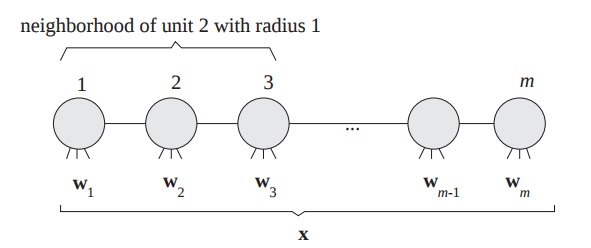
\includegraphics[height=8cm, width=8cm]{./learningAlgorithm.png}
   \caption{ Learning of the prototype}
\end{figure}


\begin{equation}
  \( w_{i} = w_{i} + \eta\phi(i,k)(\xi-w_{i}) \)
\end{equation}

Usually the neighborhoods function can be of any shape. In this context let us
assume the function is a radius of length (\r)\. Then all the unit within
neighborhood of \hl{\textbf{winner}} neuron will be updated.\\  

\begin{itemize}
   \item As th e weight converges every iteration the neighborhood function
    \(\phi(i,k)\) is shrinked.
  \item The learning rate \(\eta\) is also decreased after every iteration depending on
    the conve rgence of the weight neuron. 
\end{itemize}

\section{Program Output by the given Source Code and Analysis}
The provided source code has been modified slightly for input dimension. The
given source code was tested for the \textbf{Iris Data Set} and projected to a
two dimentional space depicted in the figure 2. Both of the image are output of
same dataset with different iternation number. 


\begin{figure}
\centering
\begin{subfigure}{0.5\textwidth}
  \centering
  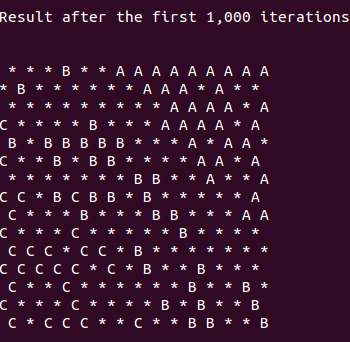
\includegraphics[width=.5\linewidth]{i2.png}
   \caption{Output after 1000 iteration}
\end{subfigure}%
\begin{subfigure}{0.5\textwidth}
   \centering
  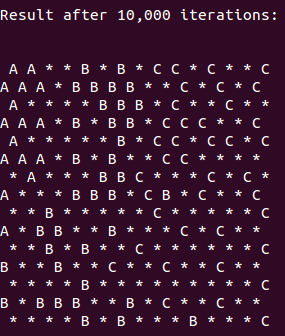
\includegraphics[width=0.5\linewidth]{i3.png}
  \caption{Output after 10,000 iteration}
\end{subfigure}
\end{figure}

We can observe from figure 1(a,b) that the program has projected the 3 class of
Iris into there repsective clusteres in two dimentional space. Three of the
class are denoted as \textbf{A,B and C}. 

\section{Visuilizing in 2D-plan with Python Visuilization tools}


For a better visuilization of the input space and output space we have
implemented the proposed problem in python with different dataset such as,
\textbf{Iris Data}, \textbf{digits}. Since python is equipped with better
visuilization tools we leveraged it and found some clear idea. 

\subsection{Iris Data Set}

\begin{figure}
  \centering
  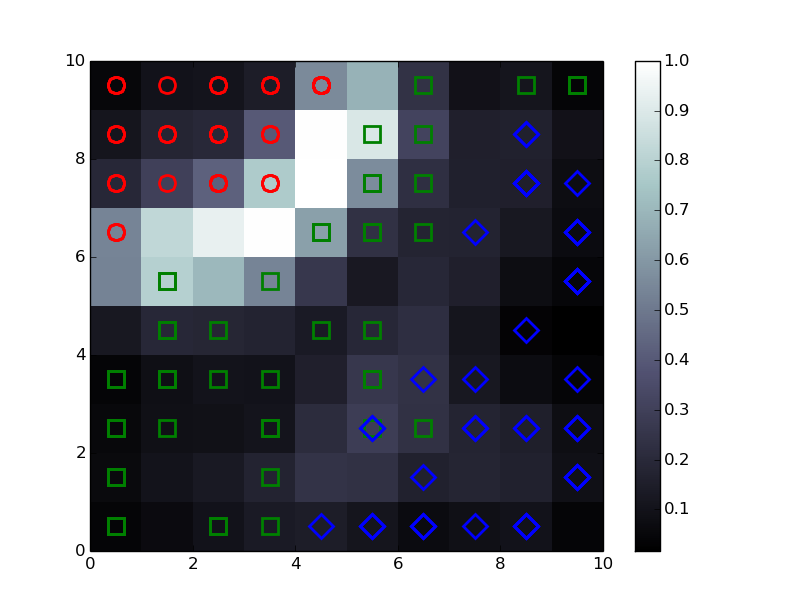
\includegraphics[height=10cm, width=10cm]{i4.png}
  \caption{Iris data Visuilized in 2D Plan}
\end{figure}

\begin{figure}
  \centering
  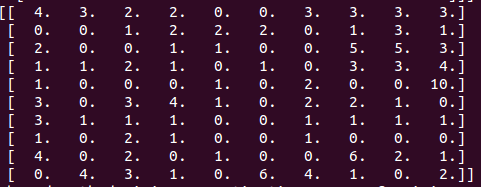
\includegraphics[height=10cm, width=10cm]{i5.png}
  \caption{The number of times winner neuron fires for each input}
\end{figure}

About 150 of the data was mapped in the 2d plane. The distance bar depicts how
far is the mapped data away from the winner neuron. Also, the number of times
winner neuron fires in shown in the figure 3.


\subsection{Digits}

The experiment with digits was done using 5 different digits. Each digit has 64
features, that is 64 dimensions. We have used the Mini self organizing map
library and project these digits in 2 dimensional surface as depicted in figure 

\begin{figure}
  \centering
  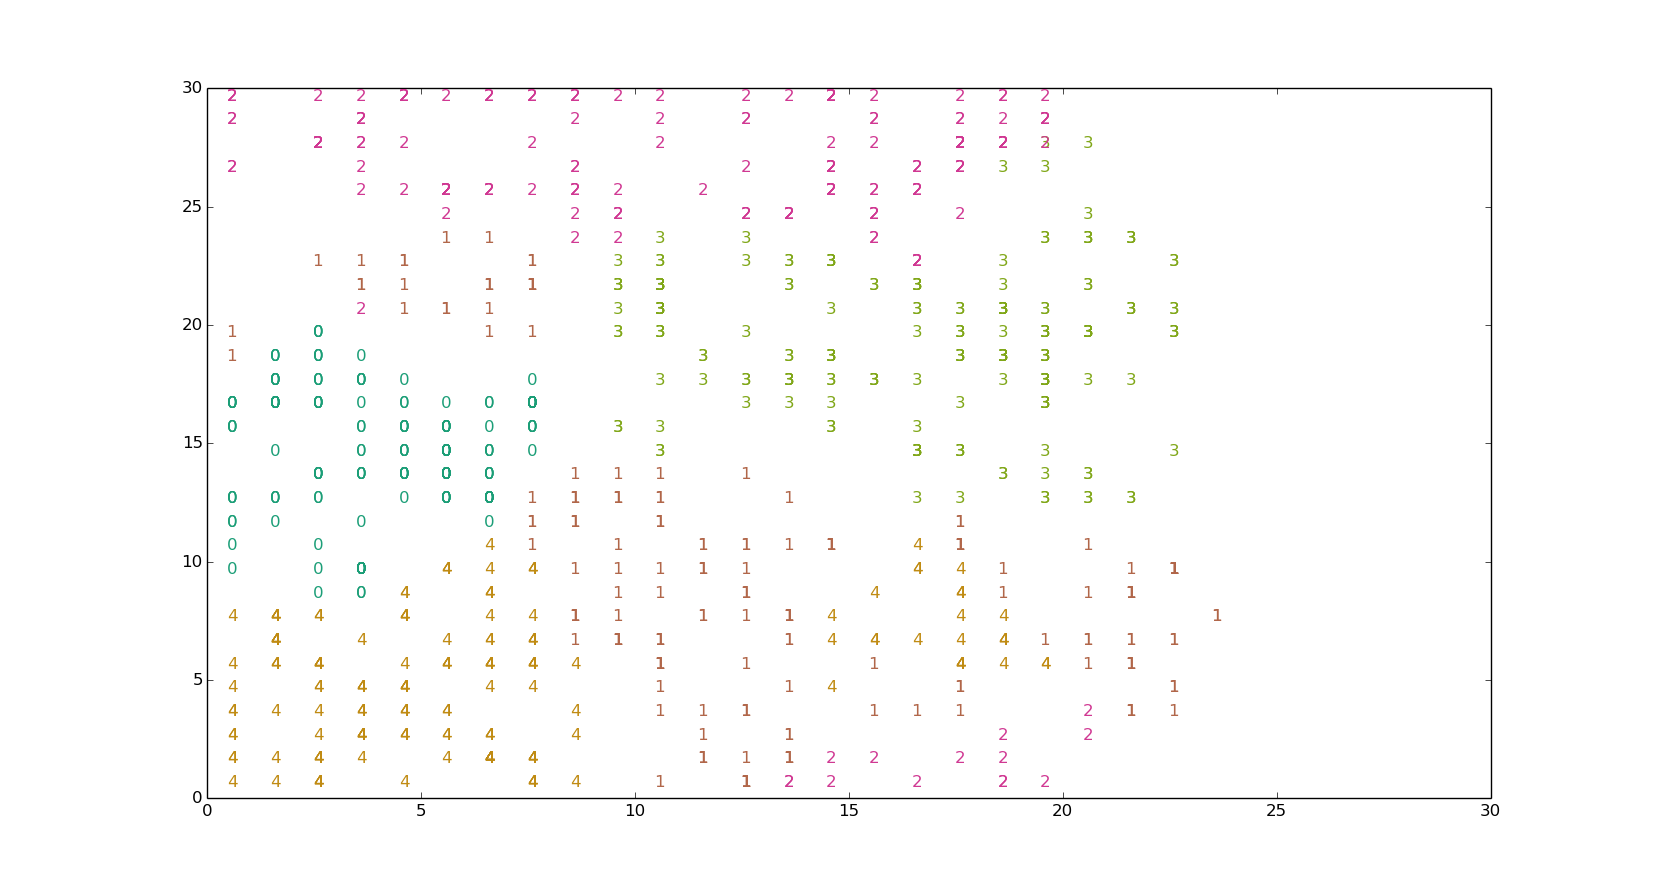
\includegraphics[height=10cm, width=10cm]{i6.png}
  \caption{Digits datasets projected on 2D-plane using SOFM}
\end{figure}


\section{Experiment with Image to demonstrate Learning Vector Quantization}
\subsection{Learning Vector Quantization}
The learning vector qualization is the supervised version of vector
qualization. We applied this method for image quantization which  alligns
with the property of Kohonen network. An image is fed as input. As output we
found compressed and clustered element of the image. Although the image is not
clear but it is understandable. 





\begin{figure}
  \centering
  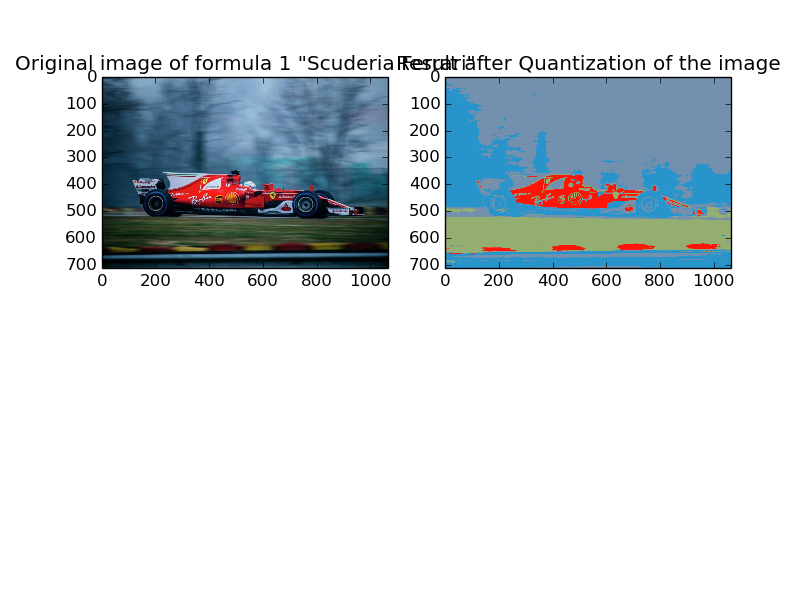
\includegraphics[height=10cm, width=10cm]{i7.png}
  \caption{Original Image in the left, and quantized image in the right with
  the help Self Organizing Map}
\end{figure}

We can see from the image that, the Self organizing network quantized the
important detail of the image. It learns the similar colors and mapped them in
to their respective places. 




\textit{The source code for the program has been attached with the file.}




\end{document}

